\documentclass[12pt]{article}
%#Scott Pratt 2022
\usepackage{subfiles}
\usepackage{indentfirst}
\usepackage{graphicx}
%\usepackage[anythingbreaks,hyphenbreaks]{breakurl}
\usepackage[anythingbreaks,hyphenbreaks]{xurl}
%\usepackage{pdfsync}
\usepackage{amssymb}
\usepackage{amsmath}
\usepackage{bm}
\usepackage[utf8]{inputenc}
\numberwithin{equation}{section} 
\numberwithin{figure}{section} 
\usepackage[small,bf]{caption}
%\usepackage{fontspec}
%\usepackage{textcomp}
%\usepackage{color}
\usepackage{fancyhdr}
\setlength{\headheight}{16pt}
%\usepackage[headheight=110pt]{geometry}
\usepackage{bm}

\usepackage[most]{tcolorbox}
\tcbset{
frame code={}
center title,
left=0pt,
right=0pt,
top=0pt,
bottom=0pt,
colback=gray!25,
colframe=white,
width=\dimexpr\textwidth\relax,
enlarge left by=0mm,
boxsep=5pt,
arc=0pt,outer arc=0pt,
}
\newcounter{examplecounter}
\counterwithin{examplecounter}{section}
\setcounter{examplecounter}{0}
\newcommand{\example}[2]{\begin{tcolorbox}[breakable,enhanced]
\refstepcounter{examplecounter}{
\bf Example \arabic{section}.\arabic{examplecounter}:}~~{\bf #1}\\
{#2}
\end{tcolorbox}
}

%\newcommand{\exampleend}{
%\begin{samepage}
%\nopagebreak\noindent\rule{\textwidth}{1pt}
%\end{samepage}
%}

%\usepackage{silence}
%\WarningFilter{hyperref}{Token not allowed in a PDF String}

\newcommand\eqnumber{\addtocounter{equation}{1}\tag{\theequation}}

\newcommand{\solution}[1]{ }

\usepackage{comment}
\parskip 4pt
\parindent 10pt

%\newcommand{\bm}{\boldmath}
\boldmath

%
\begin{document}


\begin{titlepage}
   \begin{center}
       \vspace*{1cm}

       \textbf{User Manual}

       \vspace{2.0cm}

       \textbf{Scott Pratt, Eren Erdogan, Ekaksh Kataria}
       
       \vfill
            
       \vspace{0.8cm}
     
       
\includegraphics[width=0.4\textwidth]{FRIB_logo.png}
            
            
   \end{center}
\end{titlepage}

\tableofcontents

\newpage


\section{Motivation}


 % Motivation behind this program and its uses

 A prequsie to the entire emulator is the assumtion that the user has a basinc understaing of C and C++. 


\section{Getting Started}\label{sec:simplex}

\subsection{Installation}

For installing, one should do a git pull to the smooth emulator using the link and using commands git pull with the fooling documentation in the terminal by creating a directory in which one wants to work. Important note to mentions is that the emulator works in UNIX, Mac-OS or Linux and is not supported by Windows OS

\begin{description}
\item[Step 0 : Prerequisites] 
\end{description}

Smooth Emulator uses some extra libraries that need to be installed to your computer, and added to the PATH environment for it to work. These libraries are:

\begin{itemize}
    \item CMake
    \item Eigen3
    \item GSL
\end{itemize}

CMake is an open-source, cross-platform build system that helps automate the process of building, testing, and packaging software projects. It provides a simple and efficient way to generate platform-specific build files (e.g., Makefiles, Visual Studio projects) from a platform-independent configuration.

Visit the CMake website (https://cmake.org/) to download it.\\

Eigen is a lightweight C++ template library for vector and matrix math, a.k.a. linear algebra. The program uses Eigen's matrix solvers to find solutions to certain problems.

Visit the Eigen website (https://eigen.tuxfamily.org/dox/) to download it.\\

The GNU Scientific Library (GSL) is a numerical library for C and C++ programmers. The library provides a wide range of mathematical routines such as random number generators, special functions and least-squares fitting. There are over 1000 functions in total with an extensive test suite.

Visit the GSL website (https://www.gnu.org/software/gsl/) to download it.\\

\begin{description}
\item[Step 1 : Making Directory and Environment Variable]
\end{description}

The first step is 2 fold, first start by creating a directory in the users computer when the user is in the .bash and calling it git\_msu using the following command 

{\tt 
\begin{verbatim}
    mkdir githome_msu 
\end{verbatim}
}

Then start by creating an environmental variable which is done by adding the command in the Unix shell and for Mac-OS do the following commands and add the it in the zsh's user configuration for interactive shells.  

{\tt 
\begin{verbatim}
    e .zshrc
\end{verbatim}
}

After opening the .zshrc file add the following command 

{\tt 
\begin{verbatim}
    export GITHOME_MSU="/Users/'username'/git"
\end{verbatim}
}

after saving the .zshrc file and restating the terminal one can make sure this works one can run the following command 

{\tt 
\begin{verbatim}
    echo ${GITHOME_MSU} 
    
    and it will output 
    
    "/Users/'username'/git"
\end{verbatim}
}

where the username is going to be varied for different users.

\begin{description}
\item[Step 2 : Downloading] 
\end{description}

After creating the git directory take the terminal window and run the following command 

{\tt 
\begin{verbatim}
    git pull https://github.com/scottedwardpratt/ 
\end{verbatim}
}

This downloads 2 directories: communities and smooth \\

Their functionality is mentioned in the structure section. 
After pulling one should get familiar with the environment created and the structure. This program runs on any C++ and c editors such as Atom, Visual Studio etc. \\ 

After downloading create a directory in the smooth directory such as projectX and using the git copy command, copy the items in the scottrun directory into the new directory using the following command when the terminal is in the project directory.



\begin{description}
\item[Step 2 : Making a Project Directory] 
\end{description}
{\tt 
\begin{verbatim}
    cp -r ../template/model* . 
\end{verbatim}
}
     
This will set up the directory structure for use.  \\ 

The user should also be informed about CMake. 

Once the installation is complete, open a terminal or command prompt and navigate to the directory where your project's CMakeLists.txt file is located.

Run the cmake command followed by the path to the project directory. For example:

\begin{description}
\item[Step 3 : CMake]
\end{description}

{\tt 
\begin{verbatim}
    cmake /path/to/project 
\end{verbatim}
}

\\


\subsection{Structure}

The directory structure of the repository is as follows: 

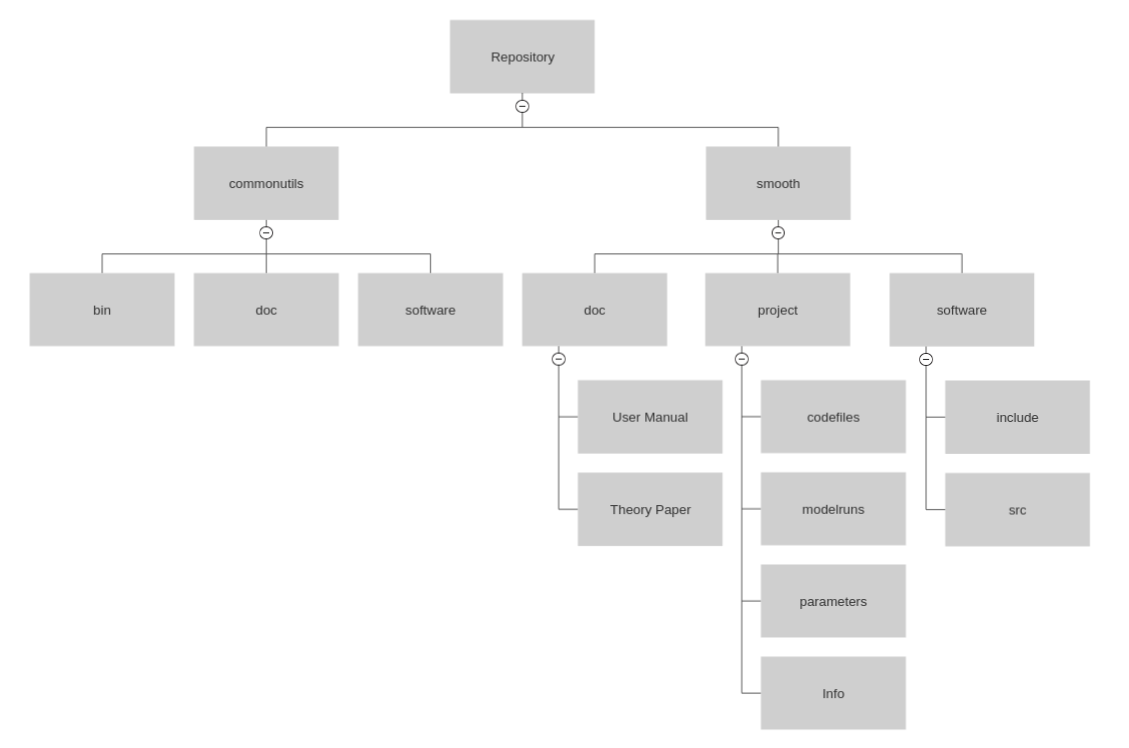
\includegraphics[width = 120mm]{Structure Tree.png}


\subsubsection{Software Directory}

The software file contains all the classes and the main functionality of the emulator. The Software file contains the two main directories, the Include directory and the source directory called src.

\subsubsection{Include Directory}

This directory contains all the header files. The header files contain a set of predefined library functions and newly defined classes for the different functions used in the emulator code, the header files have the .h extension and the C prepossessing directive "\#include" is used to include a header file that we want to use in our program.

\subsubsection{Source Directory (Src)}

This directory has the main functionality of the entire emulator as .cc files and contains the classes for each step with different constructors. The .cc files call the .h file using the "\#include" functionality and then define each class with different initial values, different methods and constructors. 

This separation of the .h and .cc files helps since one can see the different constructors defined in the .h files and one can trace them to the .cc to gain knowledge of the functionality of that particular constructor.

The .cc files are listed and briefly described below and their details will be discussed in detail in section 5. 

\subsubsection{Project Directory}

The project directory is where the emulator works. There are files in this directory: 


\begin{description}
\item[Template Project Directory] \
\\
\ 1. simplex.cc \\
\ This cc helps in choosing the training points and making the model parameters and creates the model run directory using the prior info for the simplex \\

\ 2. fakemodel.cc \\

\ The fakemodel.cc is a template used to represent a potential model. It will be replaced by the actual model created by the user. \\ 

\ 3. smoothy.cc \\

\ This cc files read in the parameter files and reads in the training point info from the simplex and tune the function Y values and generate the coefficient for each observable and make a directory of the possible coefficient values \\

\ 4. smoothy\_readcoefficients.cc \\

This cc file reads in the coefficient files and reads in the training info from the simplex and tests the samples from the emulator at the training points. 


\end{description}

The order in how the code works is mentioned in the next section 


\subsection{Usage}

The user is required to have some knowledge of C++ in order to write a routine program that calls methods from the software directory for their needs. Some example codes can be viewed in the template directory.

%Appendix for Parameter Map
\section{Parameter Map}

\ The emulator parameter map is the file user changes in order to use and optimize the code according to the model the user has and the output user is expecting. The parameters described below can be found in the parameter directory and in the file emulator\_parameter.txt. \\



\begin{tabular}{ |p{8cm}||p{6cm}|  }
 \hline
 \multicolumn{2}{|c|}{Parameter List} \\
 \hline
 Parameter Name & Uses\\
 \hline
 SmoothEmulator\_NPars   & The Number of parameters is     \\
 SmoothEmulator\_NTrainingPts &   Number of Training points that functions tunes from.   \\
 SmoothEmulator\_SigmaA   & Range value of the function \\
 SmoothEmulator\_SigmaYMin   & DZ \\
 SmoothEmulator\_NMC &   Number of Mote Carlo Simulations to run  \\
 SmoothEmulator\_NASample & Number of Coefficient samples    \\
 SmoothEmulator\_MCStepSize & Monte Carlo Step Size for each step in the parameter space   \\
 SmoothEmulator\_MCSigmaAStepSize & Monte Carlo Step Size for each step of variance in the parameter space  \\
 SmoothEmulator\_TuneChooseMCMC & AO  \\
 SmoothEmulator\_UseSigmaYRreal & AO  \\
 SmoothEmulator\_ConstrainA0 & AO  \\
 SmoothEmulator\_CutoffA & AO  \\
 SmoothEmulator\_LAMBDA & AO  \\
 SmoothEmulator\_ModelRunDirName & AO  \\
 SmoothEmulator\_CoefficientsDirName  & AO  \\
 Smooth\_MAXRANK & AO  \\
 Smooth\_UseRFactor & AO  \\
 Simplex\_TrainType & Determines the training type  \\
 Simplex\_RTrain & AO  \\
 

 
 \hline
\end{tabular}


\section{Simplex}

\subsection{Summary}
The functionalities of the simplex class are training point generation and writing model parameters to all the run files. 

\subsection{Training Point Generation}


\section{Tuning the Emulator}

\subsection{Summary}

From the motivation, we can interpret that the purpose of the emulator is to reproduce the model reasonably away from the training points and the goal is to focus on a particular class of functions that are smooth. 

The emulator has a specific functional form with numerous coefficients denoted as $A_{\vec{n}}$. The theory of steps illustrated on how to constrain the emulator is mentioned in the theory section below. 

After Running the simplex.cc file we output the model\_par.txt files for each run using the prior information using the number of parameters sent from the model\_parameter.txt file from the info directory and use the simplex to create the training points.

\subsection{Code}

For training the emulator we create the coefficient samples using the smoothy
\_writecoefficients.cc. The Functionality, how to use and the output of these files are explained below.

The fakemodel.cc is a template used to represent a potential model. It will be replaced by the actual model created by the user. The file reads in the model prior info and the observable info files from the info directory and generates the observable text files in the run directory. 
 
\subsection{Writing Coefficients}

This code is responsible for invoking the primary functionality that adjusts the training points for the model. It generates coefficient samples, which are then organized in a coefficient directory within the project directory. The directory contains information about each observable and samples of various coefficient values. The following constructors are used to accomplish this task:

\begin{description}
\item[Step 1 : Reading the Training Information]
\end{description}

{\tt 
\begin{verbatim}
    master.ReadTrainingInfo(); 
\end{verbatim}
}

This is called from the trainnginfo.cc file and takes in the run directory name and reads in the values from each run directory and stores the values of the observables and the parameters values and stores in the current code. 

\begin{description}
\item[Step 2 : Tuning in all functions(Y). ]
\end{description}

{\tt 
\begin{verbatim}
    master.TuneAllY(); 
\end{verbatim}
}

This is called from the emulator.cc file and according to the constraints the rules explained above attempt to find the optimal set of coefficients that best match the training data. This code defines a function TuneMCMC within the class CSmoothEmulator.

The purpose of this function is to perform a Markov Chain Monte Carlo (MCMC) parameter tuning process to optimize some coefficients of a smooth emulator. 

The code attempts to find the best set of coefficients that maximize the log probability of the emulator given some training data. \\

\ 1. Adaptive Step Size:

The algorithm employs an adaptive step size (stepsize) for each parameter during the trial update process. The step size depends on SigmaA, MCStepSize, and a constant LAMBDA.

The MCStepSize and MCSigmaAStepSize are tunable parameters that control the magnitude of the parameter updates. \\

\ 2. Acceptance Criteria:

If the trial log-likelihood (logPTrial) is higher than the current log-likelihood (logP), the trial parameter set is accepted as the new current parameter set, and the algorithm moves to the next iteration.

If the trial log-likelihood is lower, the algorithm applies the Metropolis-Hastings acceptance criterion: the trial parameter set is accepted with a probability of exp(dlp) (where dlp = logPTrial - logP).

The algorithm also keeps track of the best log-likelihood encountered so far (BestLogP). \\

\ 3. Parameter Updates and Success Count:

Successful updates are tracked using the success counter, which increments every time a trial parameter set is accepted (either unconditionally or based on the acceptance criterion). \\ 

\ 4. Final Output and Results:

After completing the specified number of iterations, the algorithm calculates the success percentage (proportion of successful updates), the final value of SigmaA, and the log-likelihood normalized by the number of degrees of freedom (Ndof) for the best parameter set (BestLogP/Ndof).

These results are displayed in the console using CLog::Info(). \\ 

\ 5. Interpreting the Results:

The success percentage gives an indication of the acceptance rate of new parameter sets during the MCMC process. A higher success rate generally indicates efficient parameter tuning.

The value of SigmaA represents the estimated uncertainty or spread in the parameter space.

The BestLogP/Ndof provides a measure of the goodness of fit achieved by the best parameter set. \\

\ 6. Optimization and Iterations:
For better parameter tuning results, you may need to experiment with different values of MCStepSize, MCSigmaAStepSize, and LAMBDA.

Increasing the number of iterations (NMC) can also improve the quality of the parameter tuning but may require more computational resources. \\

\ Overall, this code performs an MCMC parameter tuning process for the coefficients of a smooth emulator, attempting to find the optimal set of coefficients that best match the training data. The success rate, final variance (SigmaA), and log probabilities are reported for evaluation purposes. \\ 

\begin{description}
\item[Step 3 : Generating the coefficient (A) samples]
\end{description}

{\tt 
\begin{verbatim}
    master.GenerateCoefficientSamples()
\end{verbatim}
}


\ This code defines a function named GenerateASamples() within the class CSmoothEmulator. 

This function is responsible for generating multiple samples of coefficients (A) for a smooth emulator using the Markov Chain Monte Carlo (MCMC) tuning process. 

The function also updates statistics for the sampled variance (SigmaA) to calculate the average variance (SigmaAbar) over all the generated samples. 

In summary, GenerateASamples iteratively tunes the coefficients using MCMC and stores the optimized coefficient samples in a matrix for further analysis. 

It is used for the process of generating and analyzing samples for the smooth emulator.

\begin{description}
\item[Step 4: Testing the Coefficients At Training Points]
\end{description}

{\tt 
\begin{verbatim}
    master.TestAtTrainingPts(); 
\end{verbatim}
}


\ This code defines a function called TestAtTrainingPts within the class CSmoothMaster.

This function is used to assess the accuracy of a smooth emulator by comparing its predictions with the actual training data at each training point. \\ 

It Logs the comparison between the predicted value and the actual training data value for the current observable. Also, log the corresponding uncertainty. The function ends after testing all training points and observables. \\ 

The function evaluates the smooth emulator's accuracy by generating predictions for each observable at the training points and comparing these predictions with the actual training data. \\ 

The use of this function is to assess how well the smooth emulator approximates the underlying model and its ability to make accurate predictions at the training points. \\


\begin{description}
\item[Step 5: Writing Coefficients for functions. ]
\end{description}

{\tt 
\begin{verbatim}
    master.WriteCoefficientsAllY(); 
\end{verbatim}
}

\ This code defines a function called `WriteCoefficients` within the class `CSmoothEmulator`. This function is responsible for writing the coefficients of a smooth emulator to separate text files on the disk. \\

\ 1. Setting Up the CSmoothEmulator Object:

Create an instance of the CSmoothEmulator class and initialize its member variables, such as NASample, NPars, smooth $\rightarrow$ MaxRank, smooth $\rightarrow$ NCoefficients, etc., with appropriate values relevant to your specific problem. \\

\ 2. Creating Directory for Output:

The function automatically creates a directory to store the coefficient files and metadata. The directory name is specified by smoothmaster $\rightarrow$ CoefficientsDirName and is combined with the observable\_name to form the complete path.\\ 

\ 3. Writing Metadata:

The function writes metadata about the number of parameters (NPars), maximum rank (MaxRank), and total number of coefficients (NCoefficients) to a file named "meta.txt" in the created directory. \\

\ 4. Writing Coefficients for Each Sample:

For each sample generated using the GenerateASamples() function, the function writes the corresponding coefficients (parameters) to a separate file named "sampleX.txt" in the created directory, where "X" represents the sample index. 

Each file contains the coefficients for the smoothing emulator. The number of coefficients is equal to smooth->NCoefficients, and they are written in a column-wise format. \\

\ 5. Post-Processing and Analysis:

After running the WriteCoefficients() function, you will have a directory containing the coefficient files and a metadata file for the observable. \\

\ In summary, the `WriteCoefficients` function saves the coefficients of a smooth emulator to separate text files. It organizes the files in directories based on observable names, writes metadata, and stores the coefficients for each sample in a formatted manner. This enables easy storage, retrieval, and reuse of the coefficients for further analysis or model training. \\



\section{Performing the Full Model Runs}

\subsection{}

\section{MCMC}


\section{Troubleshooting}


\section{Theory}

\begin{description}
\item[Constraining the emulator] \
\\
\ 1. $M$ full model runs are conducted at different positions $\vec{\theta}_{m=1,M}$. These runs provide corresponding values $F_{m=1,M}$. \\

\ 2. The functional form of the emulator has a large number of coefficients $A_{\vec{n}}$, which exceeds the number of training points M. However, the dependence of the coefficient A is purely linear. \\

\ 3. The coefficients are enumerated as $A_c$ with $c=1\cdots C$, where $C>M$.\\

\ 4. Random values are assigned to the coefficients $A_M$ through $A_C$, excluding the first $M$ coefficients. \\

\ 5. A set of linear equations is solved to determine the values of the first $M$ coefficients. This process involves finding the coefficients that best fit the training points. \\

\ 6. A weight is applied to the values of $A$, taking into account their consistency with the prior likelihood of $A$ and the given constraints. This step helps to incorporate prior knowledge and constraints into the emulator. \\

\ 7. A representative set of A is generated, typically consisting of a dozen samples. Each sample function passes through all the training points but may deviate further from them. \\

\ 8. By averaging over $N_{\rm sample}$ sets of coefficients, a prediction for the emulator can be made at a specific point $\theta$. The $N_{\rm sample}$ points provide an estimate, and their variance represents the uncertainty associated with the emulator's prediction. \\

\end{description}




\end{document}
